% !TeX root = root.tex
% !TeX spellcheck = en_US
\section{GAP-exercise}

To solve exercises a), b) and c), we use the following GAP code:

\lstinputlisting[language=gap]{ex5.g}

For a) the function \textit{estimate1} picks 1000 elements of $S_n$ uniformly at random and determines their average order. For b) the function \textit{estimate2} picks 100 times two elements of $A_n$, calculates the order of the subgroup generated by the two elements and determines the average of the resulting orders. The function \textit{estimate3} does the same as \textit{estimate2} for $S_n$. Finally, we call the functions for all $n \in \{1, \dots, 50\}$ and store the results in the lists \textit{estOrders1}, \textit{estOrders2} and \textit{estOrders3}. We obtain the following results:

\hspace*{-1cm}
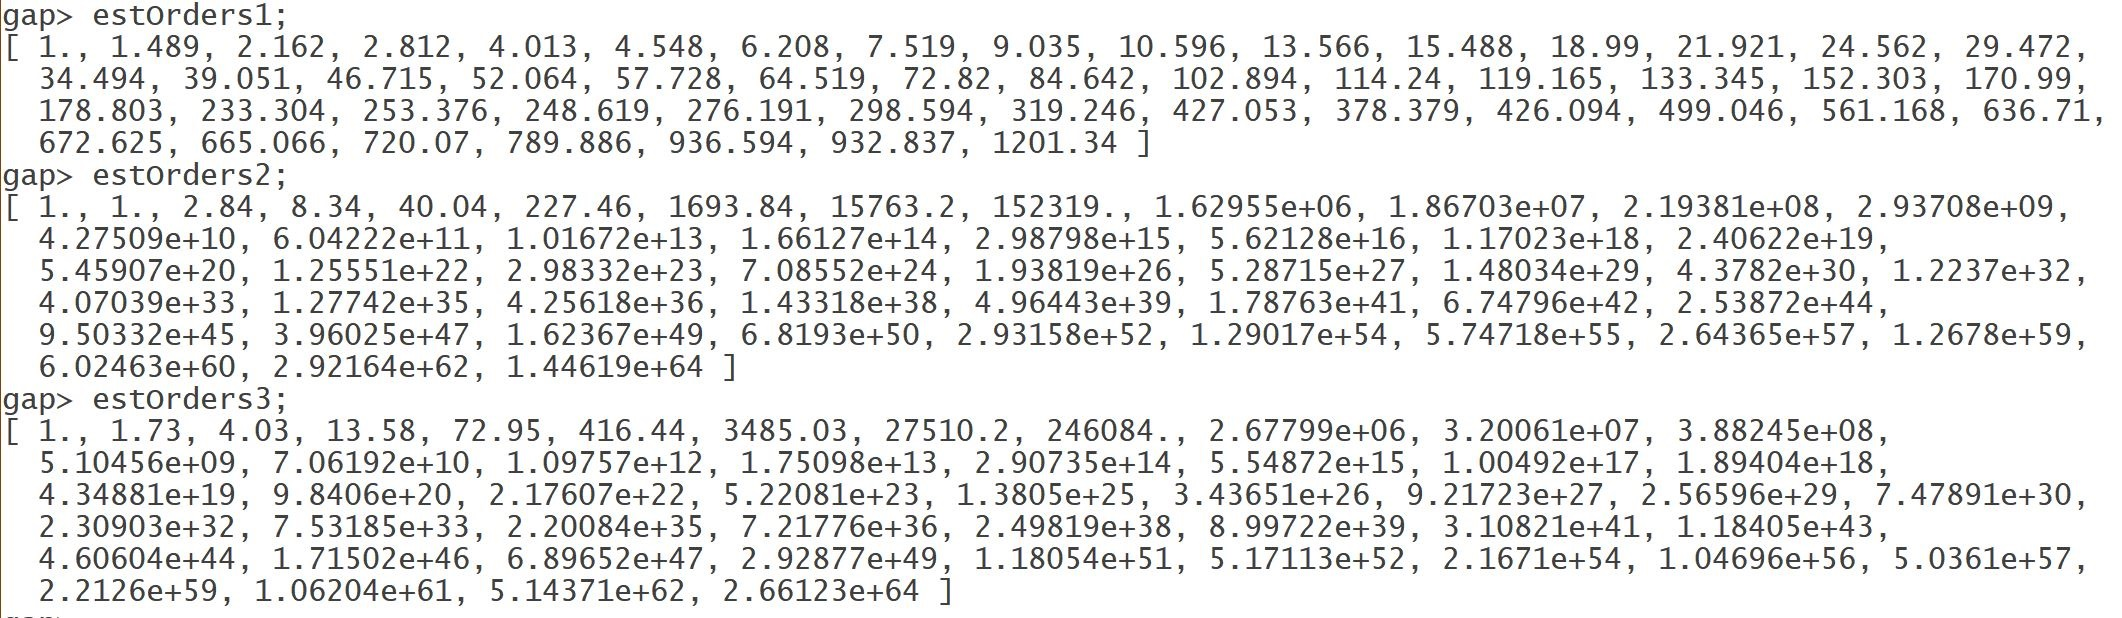
\includegraphics[width=17cm]{ex5}

The growth of the averages in a) looks polynomial in $n$. For the averages for b) and c) we observe that the values in \textit{estOrders2} are roughly half as big as the values in \textit{estOrders3}. Moreover, the growth of the averages in \textit{estOrders3} seems to be proportional to $n!$. Our conjecture for the growth of the averages for c) is $\frac{2}{3} n!$ and for b) it is $\frac{1}{3} n!$. 